\documentclass[main.tex]{subfiles}

\begin{document}
\section{Характеристики}
    \subsection{Избор}
    На дневен ред е избирането на характеристики, които отразяват идеята за разделяне на информацията за вокалния тракт
    $\mathcal{H}$ от входния сигнал $\mathcal{G}$.
    Имаме $\mathcal{Y}(\mathcal{z}) = \mathcal{G}(\mathcal{z}) \mathcal{H}(\mathcal{z})$.

    Нека вземем логаритъм от модула:
    \begin{flalign*}
        & log(|\mathcal{Y}(\mathcal{z})|) = log(|\mathcal{G}(\mathcal{z})|) + log(|\mathcal{H}(\mathcal{z})|) &&
    \end{flalign*}
    Обратното Фурие преобразувание ни дава вид във времевия домейн:
    \begin{flalign*}
        & c_y[n] = c_g[n] + c_h[n] &&
    \end{flalign*}

    Сега вече имаме сбор на входния сигнал и този на филтъра, вместо конволюция във времевия домейн.

    Да видим каква е идеята зад тези преобразувания.
    Имаме, че $\mathcal{G}(\mathcal{z})$ и $\mathcal{H}(\mathcal{z})$ са комплексни числа и взимайки модула им, губим информация за фазата. Това не е проблем, тъй като човешкото ухо не е особено чувствително към нея, затова обикновено ни трябва само амплитудата (и следователно модула). 
    
    \begin{figure}[H]%
        \centering
            \subfloat[Логаритмична скала]{%
                \label{fig:char:1:a}
                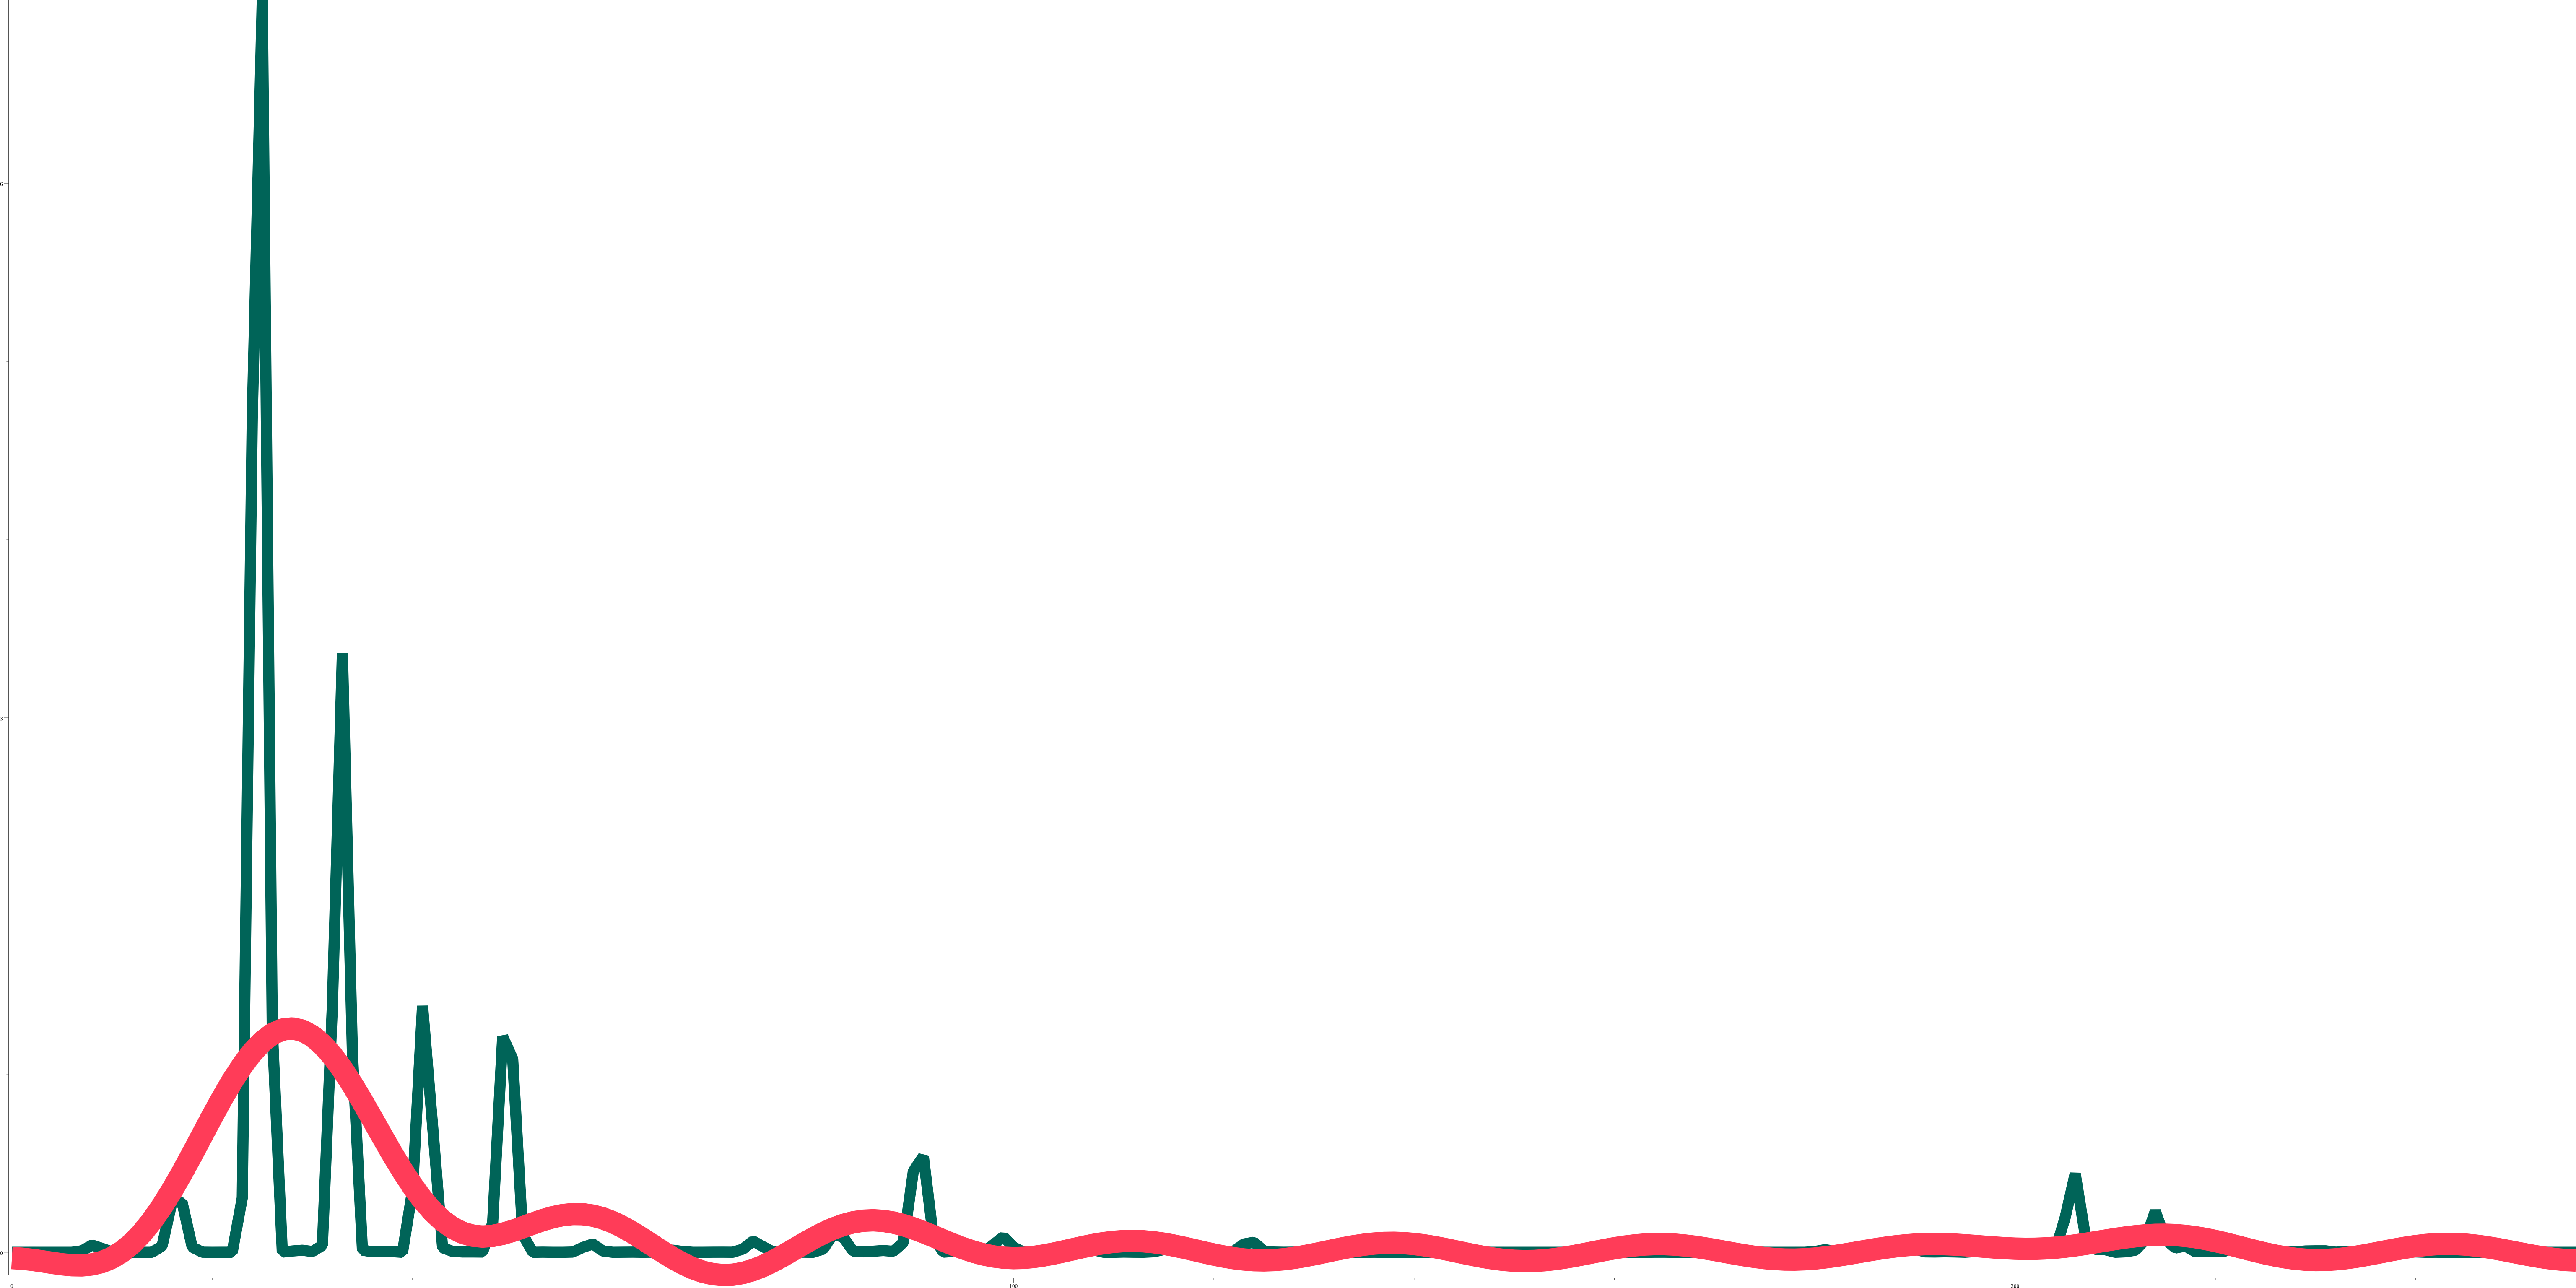
\includegraphics[width=0.40\paperwidth,valign=t]{aaaa.png}%
            }
            \hfill
            \subfloat[Логаритмична скала и логаритъм от модула]{%
                \label{fig:char:1:b}
                \includegraphics[width=0.40\paperwidth,valign=t]{aaaa_log.png}%
            }
        \caption{Графика на спектъра на сигнал, получен при произнасяне на "а-а-а-а-а"}%
        \label{fig:char:1}
    \end{figure}

    Взимането на логаритъм от модула цели да подчертае периодичността на сигнала, идващ от глотиса. 
    
    На Фигура \autoref{fig:char:1:a} се виждат пиковете, породени от
    фундаменталната честота, на която трепти глотиса, и хармоничните ѝ честоти. Поради загубата на енергията в системата за производство на реч, не всички хармонични честоти имат една и съща амплитуда.
    На Фигура \autoref{fig:char:1:b} се вижда, че взимането на логаритъм от модула помага за изравняването на хармоничните амплитуди и кара графиката да изглежда "по-периодична". 
    Сега нека разгледаме логаритмувания спектър като сигнал и му направим Фурие преобразувание до получаване на така наречения кепстър.
    Тъй като разглеждаме спектъра като сигнал, наличието на периодични амплитуди ще се преведе до пик в получения кепструм на честотата, отговаряща (горе-долу, имайки предвид джитера) на основната честота на глотиса. Информацията, която описва вокалния тракт, е с много по-малко изразена периодичност в спектъра, затова ще се запази в ниските честоти на кепстъра. Тоест $c_g[n]$  ще са коефициентите в кепстъра на високите честоти, а $c_h[n]$ в ниските. За практически цели обикновено се избират първите 13 коефициента на кепстъра. Тези коефициенти се наричат Mel Frequency Cepstral Coefficients (MFCC), където Mel скалата е логаритмична скала. Повече детайли за извличането им са описани в следващия подраздел.

    \subsection{Извличане}
    Ще извличаме характеристики от подаден аудио файл в wav формат. Първо, съдържанието на файла се прочита в масив от 64-битови float числа. Елементите на този масив се наричат дискрети (samples). Броят им зависи от честотата на дискретизация (тоест колко измервания са направени за една секунда), която обикновено е 16kHz, 44100Hz или 48kHz. Броят на дискретите определя броя на коефициентите на Фурие преобразуванието. Тъй като сигналът е реален, от \hyperref[appendix:fourier:property]{свойствата} следва, че максималната честота, която можем да измерим, е честотата на Найкуист, равна на броя дискрети върху две. Тоест - половината на честотата на дискретизация.
    Колкото е по-голяма Найкуист честотата, толкова по-добра честотна резолюция получаваме.\\
    Базирайки се на идеята, че вокалният тракт е статичен за кратък период от време, накъсваме масива на отделни застъпващи се парчета - фреймове - в рамките на които сигналът е статичен. За да се определи дължината на фрейма, трябва да се вземат предвид две неща: от една страна колкото повече дискрети имаме, толкова по-добра честотна резолюция получаваме. От друга, колкото повече дискрети взимаме, толкова по-голям е шансът да се смени конфигурацията на вокалния тракт. За да се справим с този дуализъм, компромисните стойности, които са избрани в описваната имплементация, са 25 милисекунди за дължина на фрейм и 10 милисекунди за разстояние между два последователни фрейма. Един фрейм описва една конфигурация на вокалния тракт.
    Целим да извлечем MFCC коефициенти за всеки фрейм. Това означава, че трябва да се направи Фурие преобразувание, което изисква сигналът да е периодичен, а данните във фреймовете не са. За тази цел, всеки фрейм се умножава по специално избрана функция, наречена прозорец\footnote{Прозорецът е моята врата и аз вървя към тях и ги разпитвам.}. Тази функция е нула навсякъде, освен в избран интервал, и обикновено е симетрична около средата на този интервал. Когато фреймът се умножи по прозорец със същата дължина, стойностите в краищата се нулират. Това прави полученият сигнал периодичен с период дължината на фрейма, тъй като започва в нула и завършва отново в нула.
    
    \begin{figure}[H]%
        \centering
            \subfloat[Действие на правоъгълен прозорец върху синусоида]{%
                
\includegraphics[width=0.25\paperwidth,valign=t]{rect.png}%
            }
            \hspace{2cm}
            \subfloat[Спектър на синусоида с правоъгълен прозорец]{%
                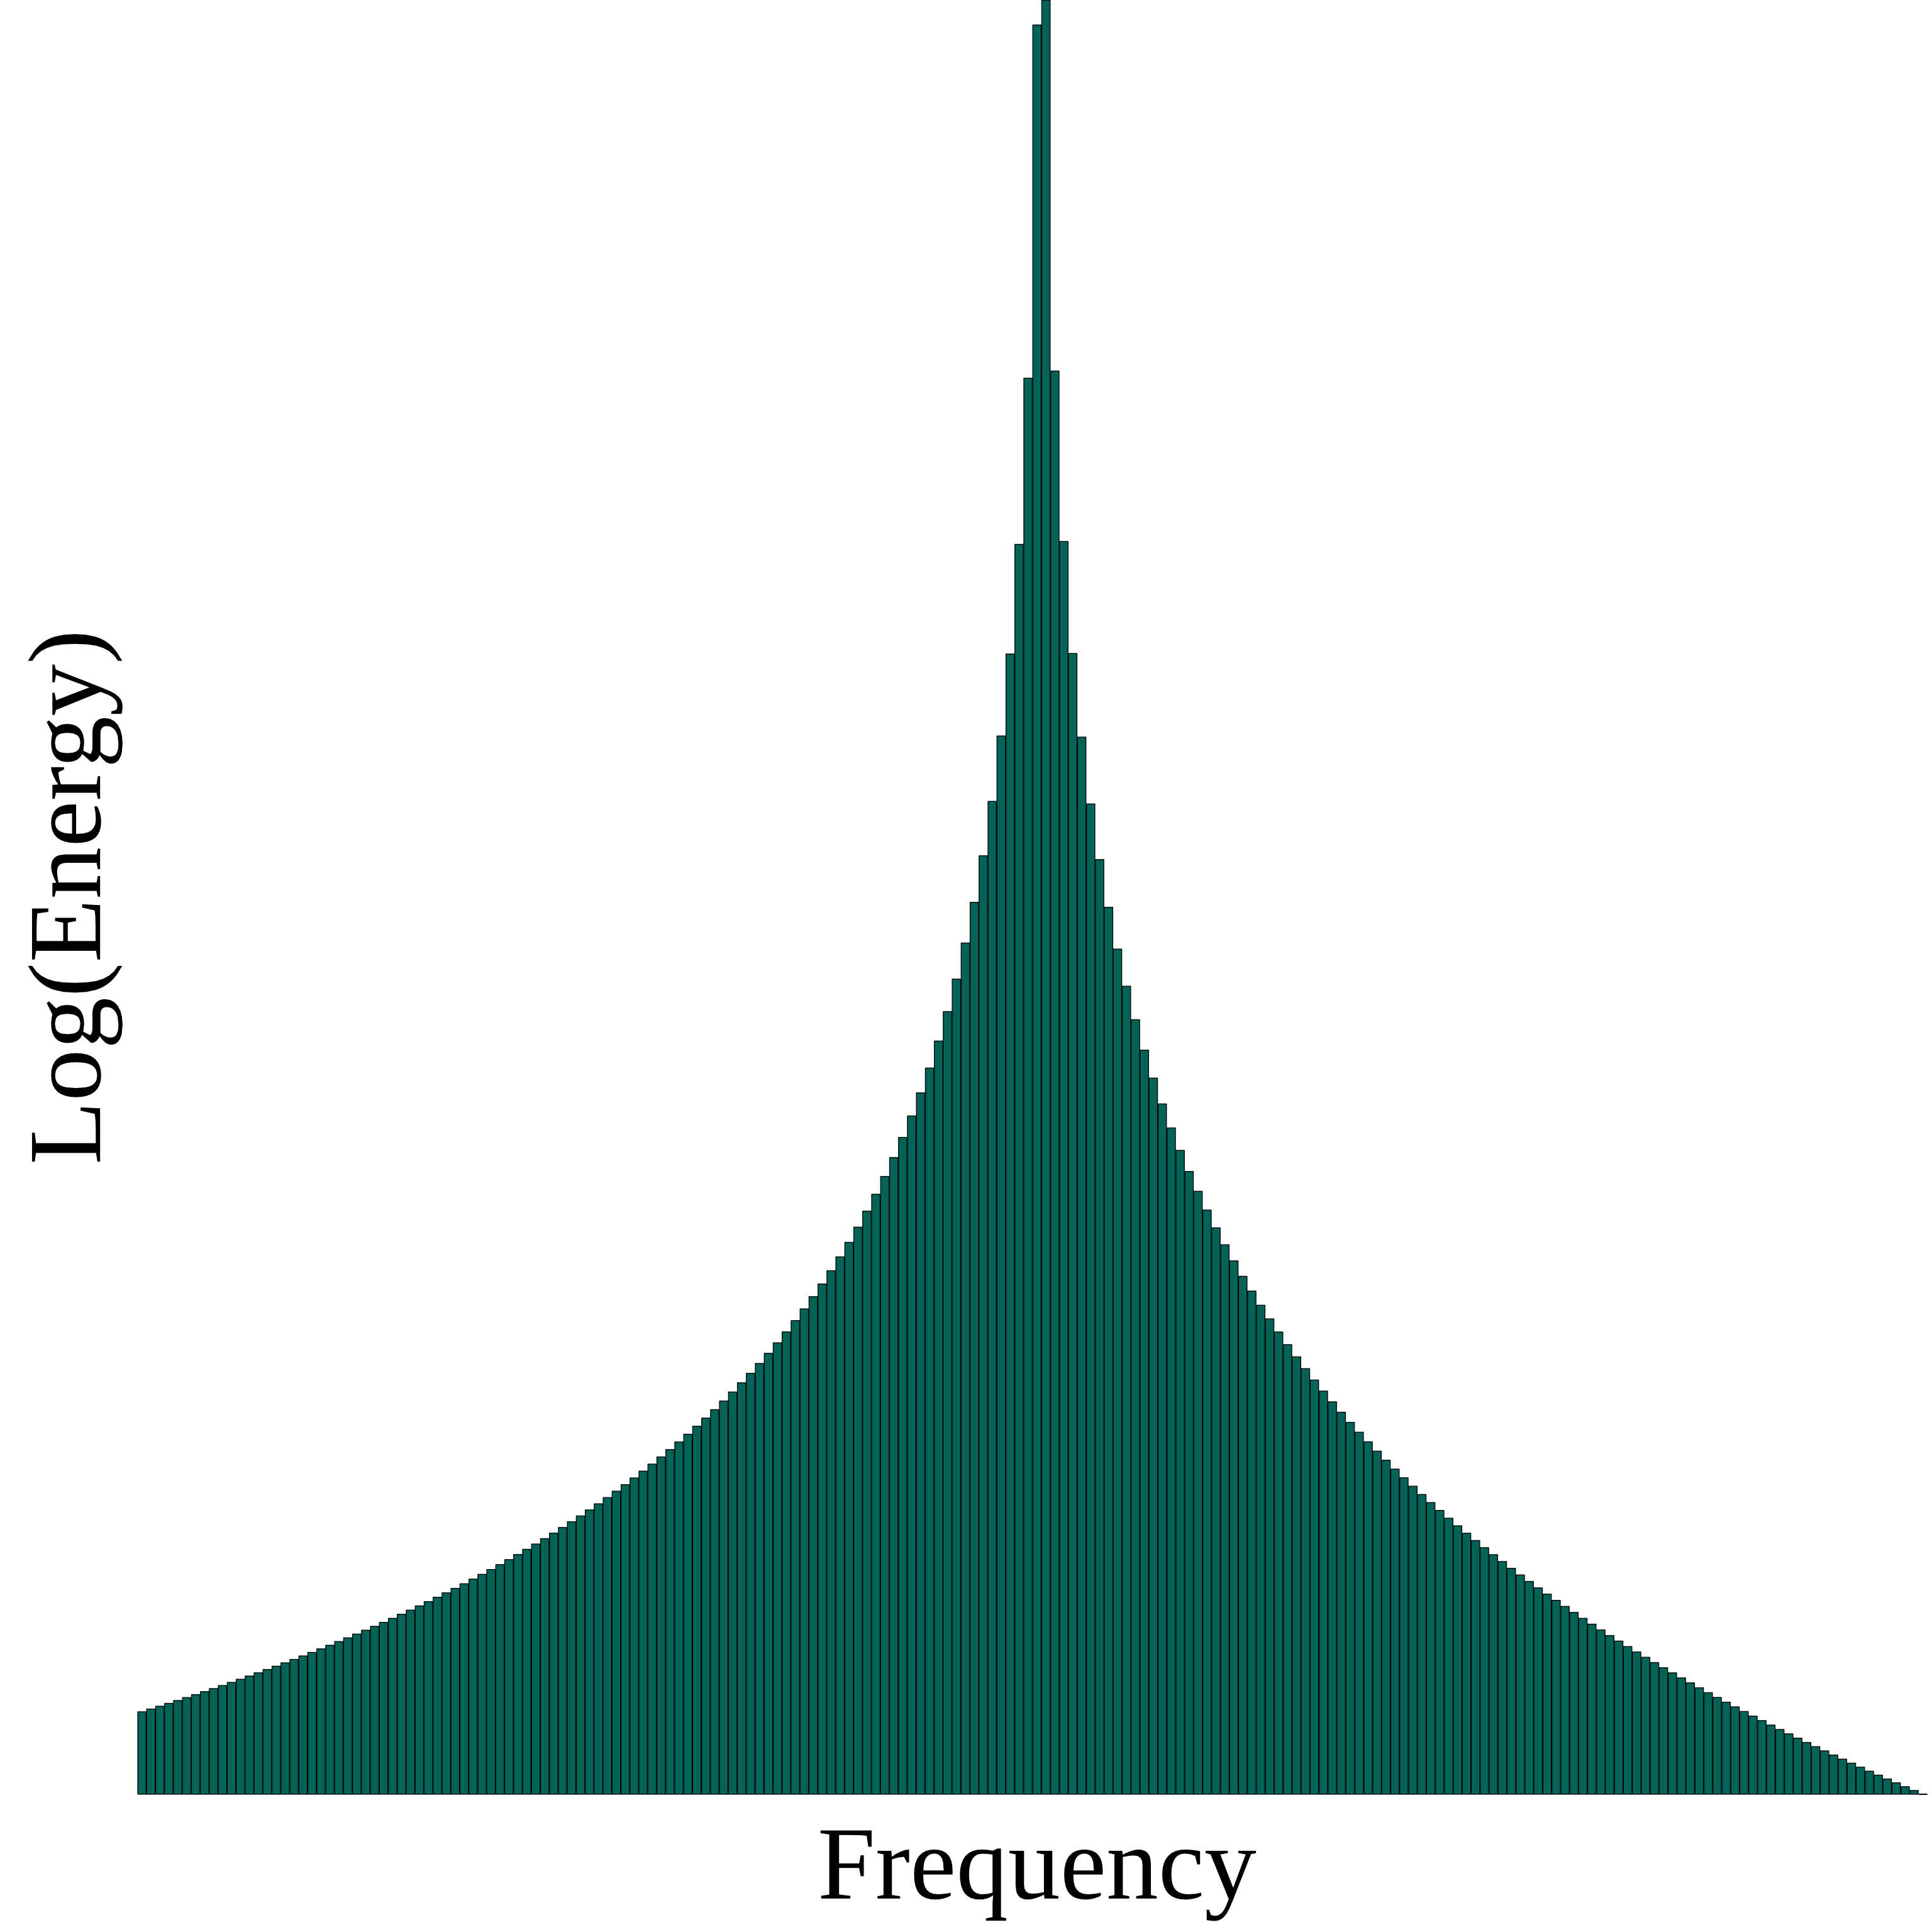
\includegraphics[width=0.25\paperwidth,valign=t]{rect_coef.png}%
            }
            \vfill
            \subfloat[Действие на прозорец на Хан върху синусоида]{%
                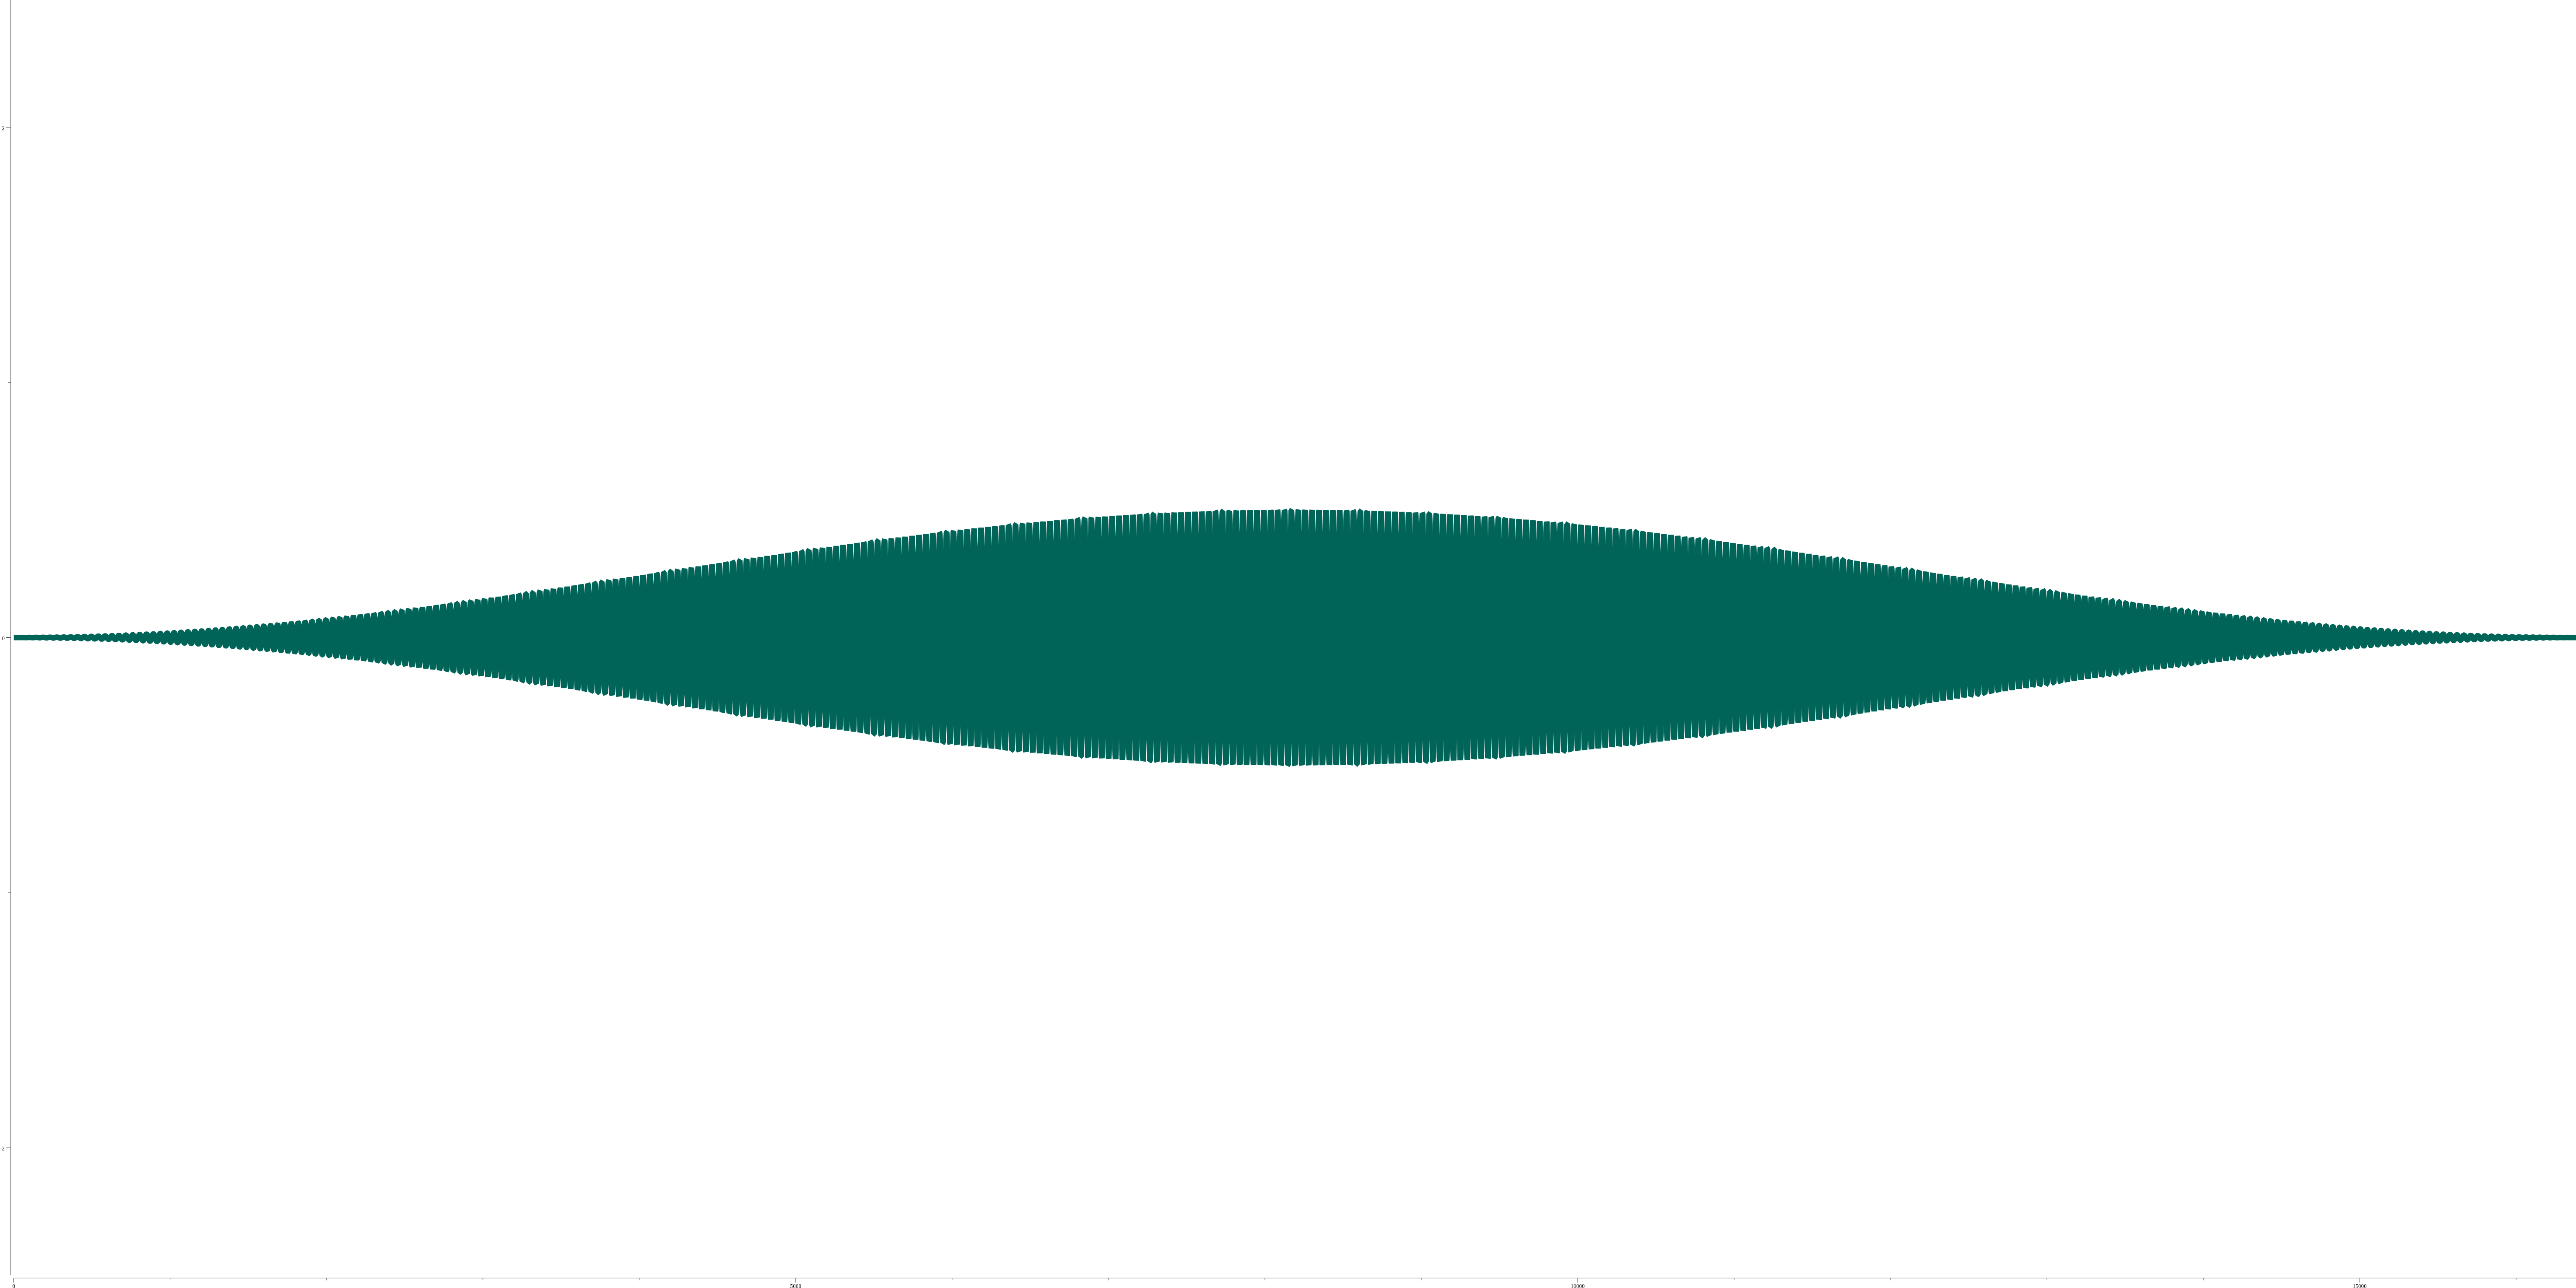
\includegraphics[width=0.25\paperwidth,valign=t]{han.png}%
            }
            \hspace{2cm}
            \subfloat[Спектър на синусоида с прозорец на Хан]{%
                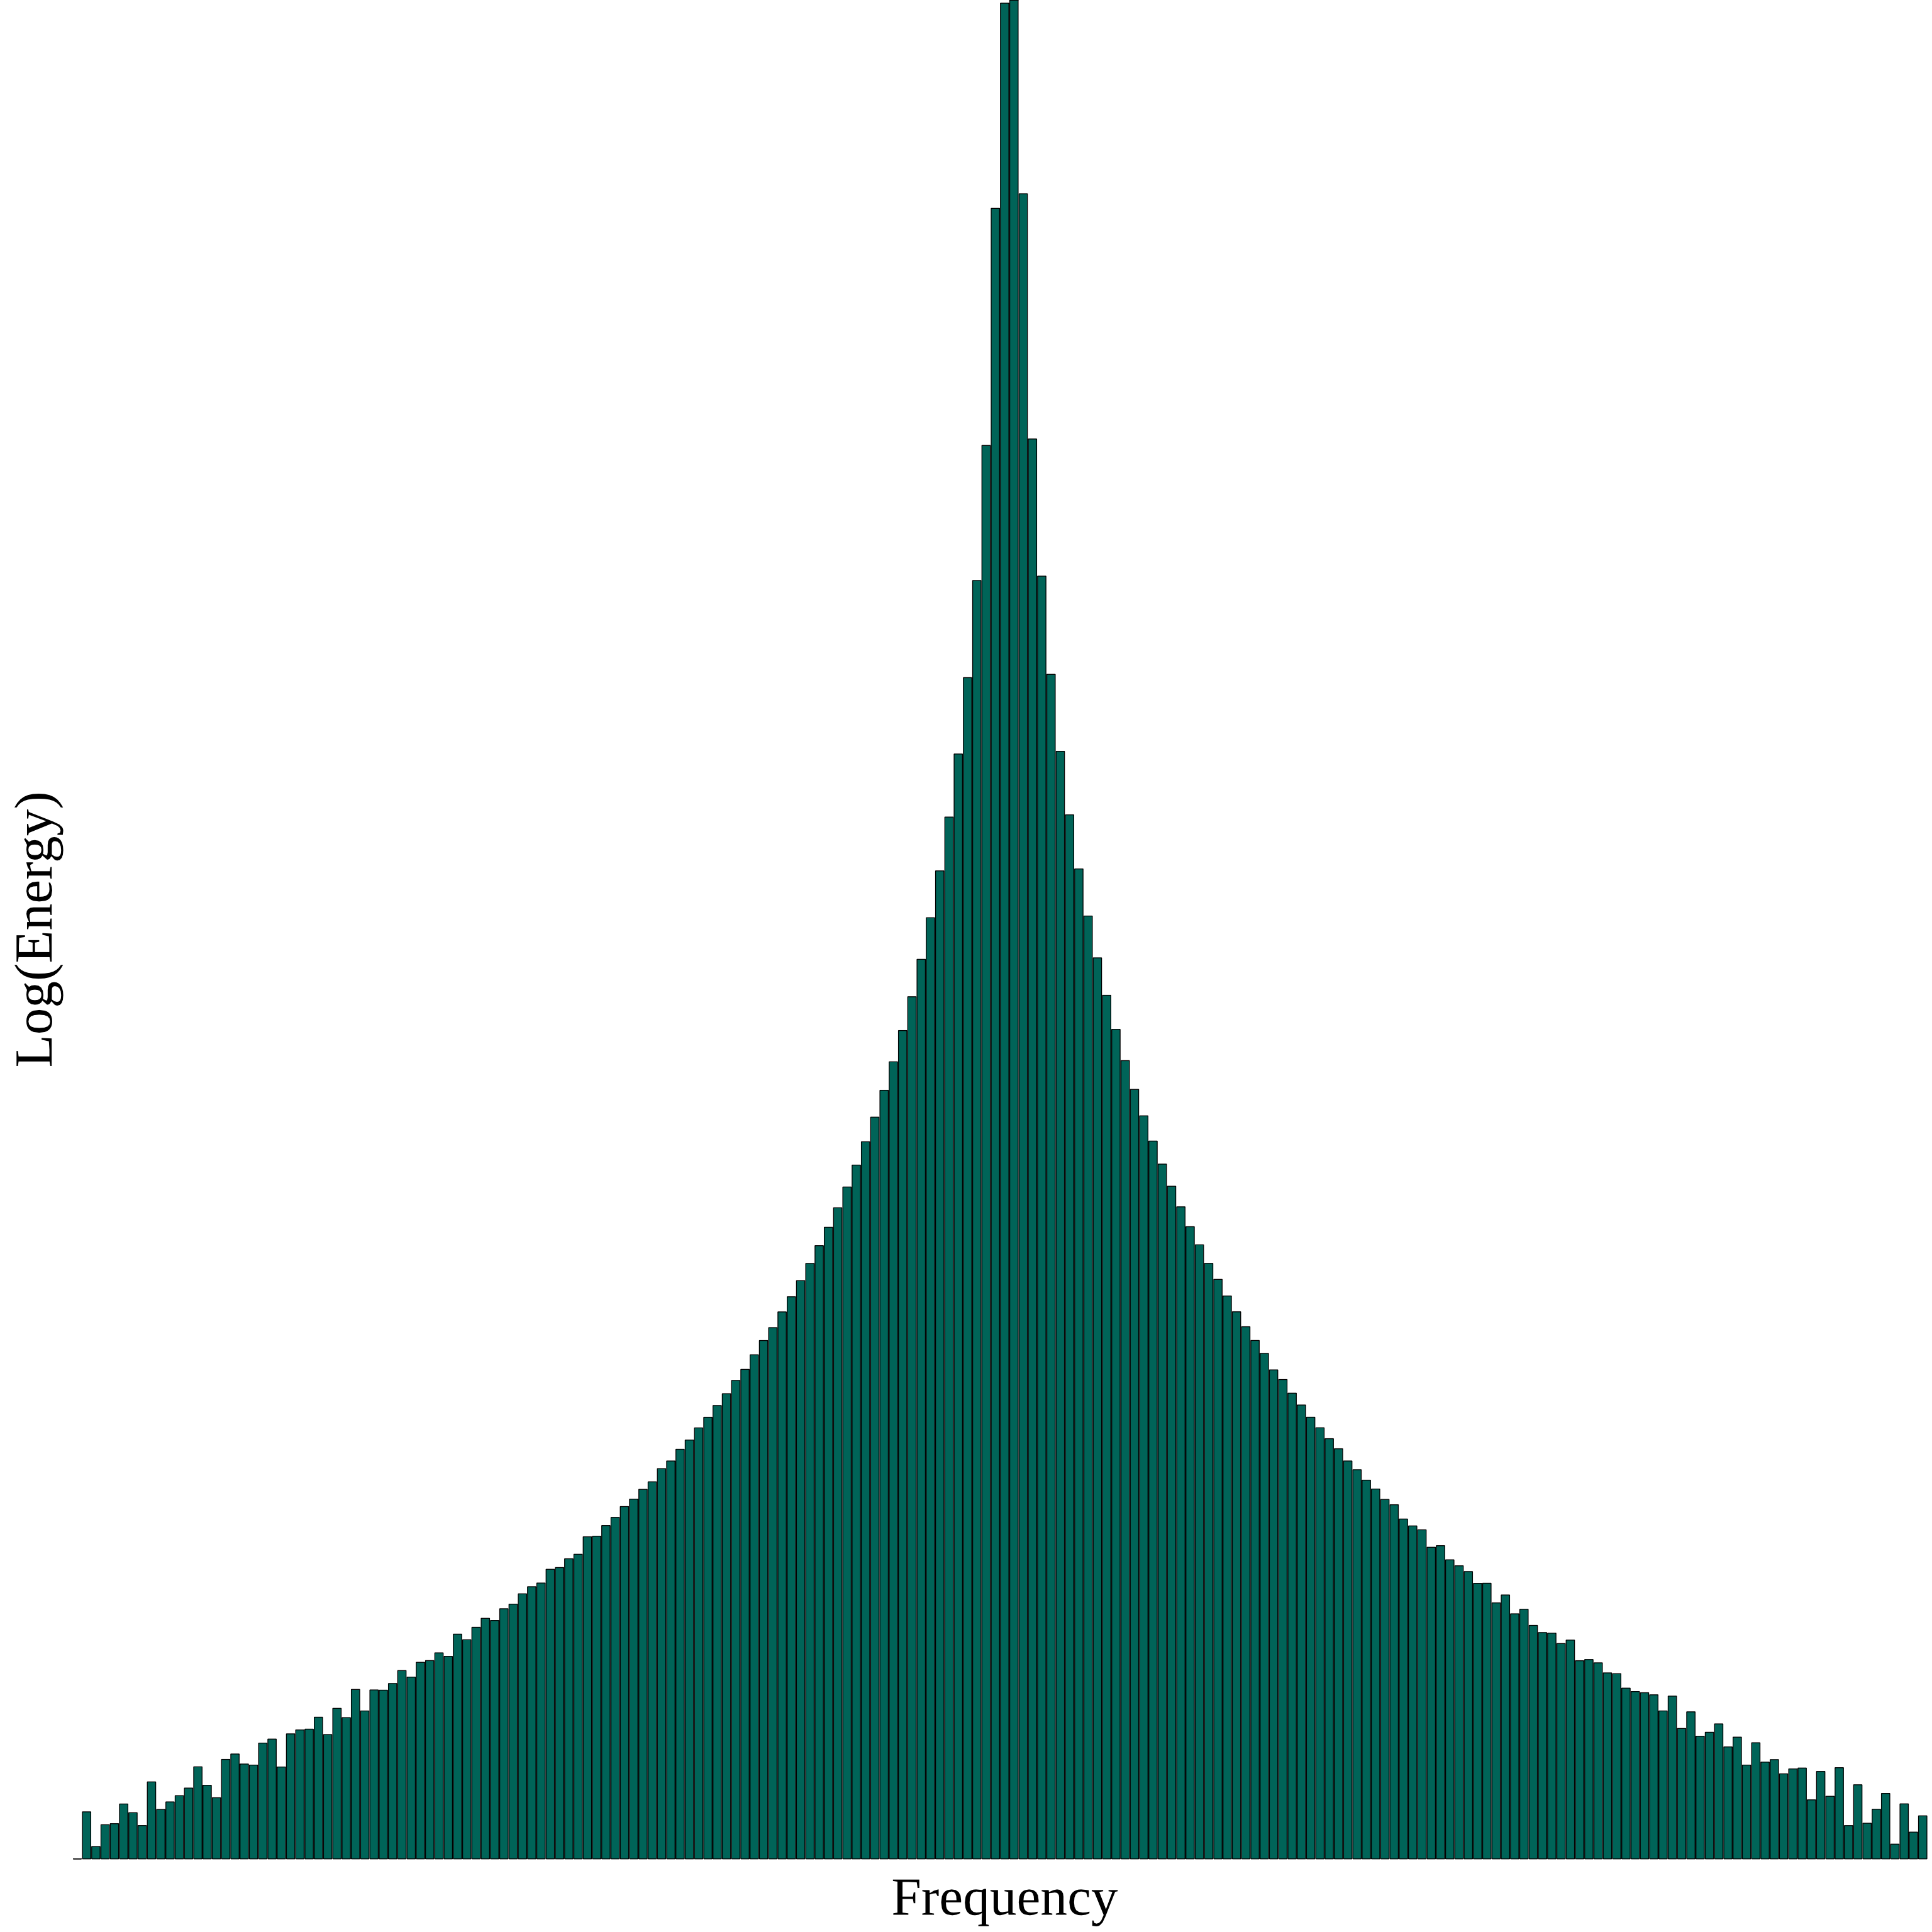
\includegraphics[width=0.25\paperwidth,valign=t]{han_coef.png}%
            }
            \vfill
            \subfloat[Действие на прозорец на Хеминг върху синусоида]{%
                
\includegraphics[width=0.25\paperwidth,valign=t]{ham.png}%
            }
            \hspace{2cm}
            \subfloat[Спектър на синусоида с прозорец на Хеминг]{%
                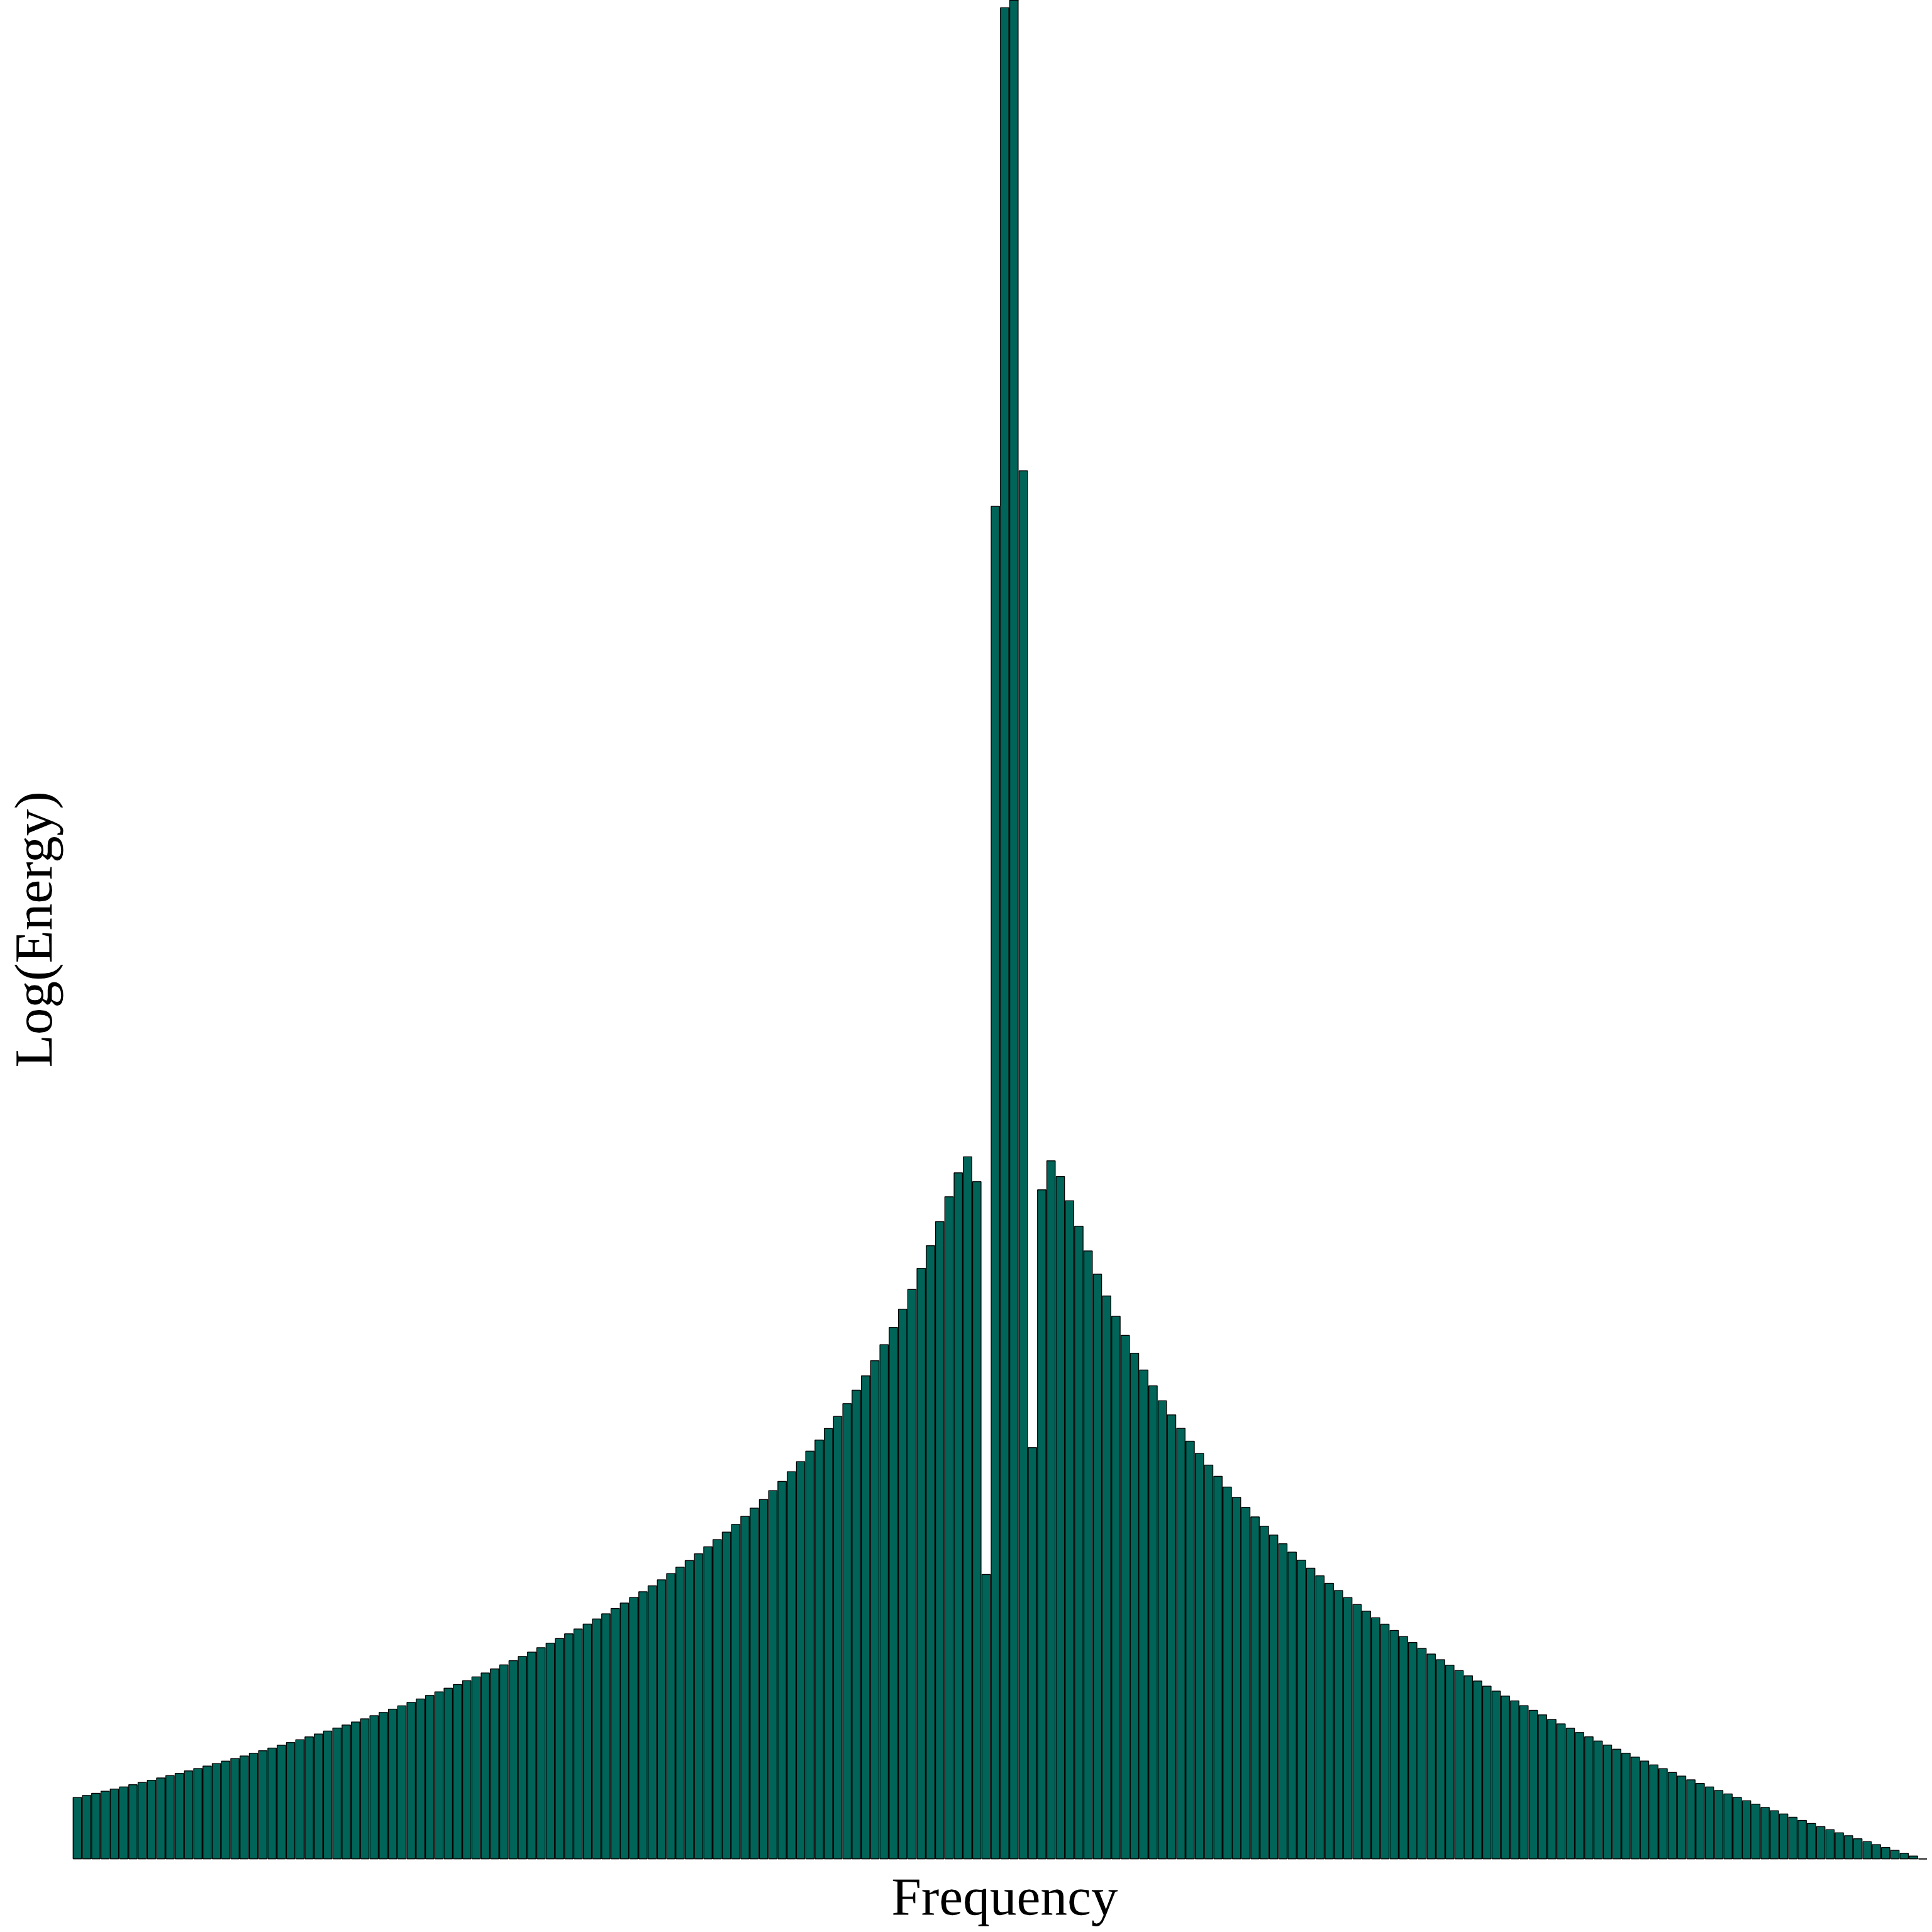
\includegraphics[width=0.25\paperwidth,valign=t]{ham_coef.png}%
            }
        \caption{Действие на често срещани прозоречни функции}%
        \label{fig:char:2}
    \end{figure}

    Най-простият прозорец, който постига желания ефект, е правоъгълният прозорец с интервал $[0, N]$, дефиниран така: 
   \[
    w_{rec}[n] = \begin{cases} 
        1, & 0\leq n \leq N \\
        0, & \text{иначе}
    \end{cases}
    \]
    Ако умножим проста синусоида по правоъгълен прозорец, се вижда на \autoref{fig:char:2}, че честотното представяне се отдалечава много от "истинското", което би трябвало да представлява единична делта функция в основната честота на синусоидата. За тази цел се въвеждат по-сложни прозоречни функции като едни от най-често ползваните са тази на Хан и тази на Хеминг, представени съответно с
    \[
    w_{hanning}[n] = \begin{cases} 
        0.5 - 0.5 \cos{\frac{2\pi n}{N}}, & 0\leq n \leq N \\
        0, & \text{иначе}
    \end{cases}\quad w_{hamming}[n] = \begin{cases} 
        0.5 - 0.5 \cos{\frac{2\pi n}{N}}, & 0\leq n \leq N \\
        0, & \text{иначе}
    \end{cases}
    \]

    Поведението им в честотния домейн може също да се види на \autoref{fig:char:2}. В описаната имплементация се ползва прозорец на Хеминг. 

    След като фреймовете вече са периодични, на всеки от тях се прави Фурие преобразувание. За да се възползваме от факта, че сигналът е реален, се използва Бързо Фурие преобразувание\footnote{на английски FFT - fast Fourier transform}.

    За да се моделира по-реалистично възприятието на звука, трябва да се отчете феноменът, че хората възприемат дразнителите чрез сетивата си логаритмично, в частност и звука. Този факт е отбелязан в закона на Вебер-Фехнер, а именно, че големината на усещането за определено дразнение е пропорционално на логаритъма на самото дразнение.
    Има различни опити да се направи скала, която по-точно да отразява човешките възприятия. Една такава е Мел скалата, която е изкуствено (емпирично) създадена. Единиците, мелове, са така избрани, че разликата между всеки два съседни да се възприема като еднаква. Връзката между меловете и честотите се задава със следната формулата:
    \begin{flalign*}
        & m = 2595 \log_{10}(1 + \frac{f}{100}) &&
    \end{flalign*}

    Втората особеност, която трябва да моделираме, е свързана с устройството на слуховия орган, тъй като целим да наподобим човешкото чуване. Главно участие има охлювчето (спирален орган), което е част от вътрешното ухо. Охлювчето е изпълнено с течност и звуковата вълна преминава през нея. По вътрешната част на охлювчето се намира така наречената базиларна мембрана, чиято дължина е покрита с рецепторни клетки - косъмчета. При преминаване на вълната през течната среда, косъмчетата се движат и предизвикват електрически сигнал, който се предава на съответните слухови неврони. Различните части на охлювчето отговарят за различни честоти (по-навътре по спиралата му са по-високите честоти). По принцип, когато два тона с различна честота стигнат до охлювчето едновременно, то ги разграничава като отделни и подава сигнал на два различни неврона. Ако тези честоти са много близки и съответно се обработват от много близки области по повърхността на охлювчето, се получава така нареченото ``слухово маскиране'', при което двата тона не могат да се различат като отделни и се подават на един и същи неврон. Такива области по повърхността на охлювчето се наричат критични области. 
    При така получените Фурие коефициенти резолюцията е твърде голяма спрямо човешките възприятия и съответно отделните честоти не могат да се разграничават от охлювчето. Тъй като честотите от една критична област се възприемат като една, то можем да разделим скалата на критични области и да акумулираме информацията в тях. Това допълнително намаля пространството, в което работим, и е удобно от изчислителна гледна точка. За практически цели често се взима броят на тези области да е 23, като обикновено се взимат застъпващи и амплитудата се умножава по триъгълен прозорец. По този начин честоти, намиращи се между две съседни критични области, допринасят към акумулираните стойности и на двете области.
    
    Като съчетаем тези две особености, получаваме застъпващи се триъгълници в Мел скалата, както е показано на \autoref{fig:char:3}, по които умножаваме сигнала. Взимаме логаритъм от енергията на сигнала, за да се подчертае периодичността на сигнала от глотиса, както обяснихме в предния раздел.
    В крайна сметка, получаваме за всеки фрейм по 23 коефициента, всеки от които стои пред акумулираните логаритми от енергии на честоти в дадена критична област.

    \begin{figure}[H]
        \centering
        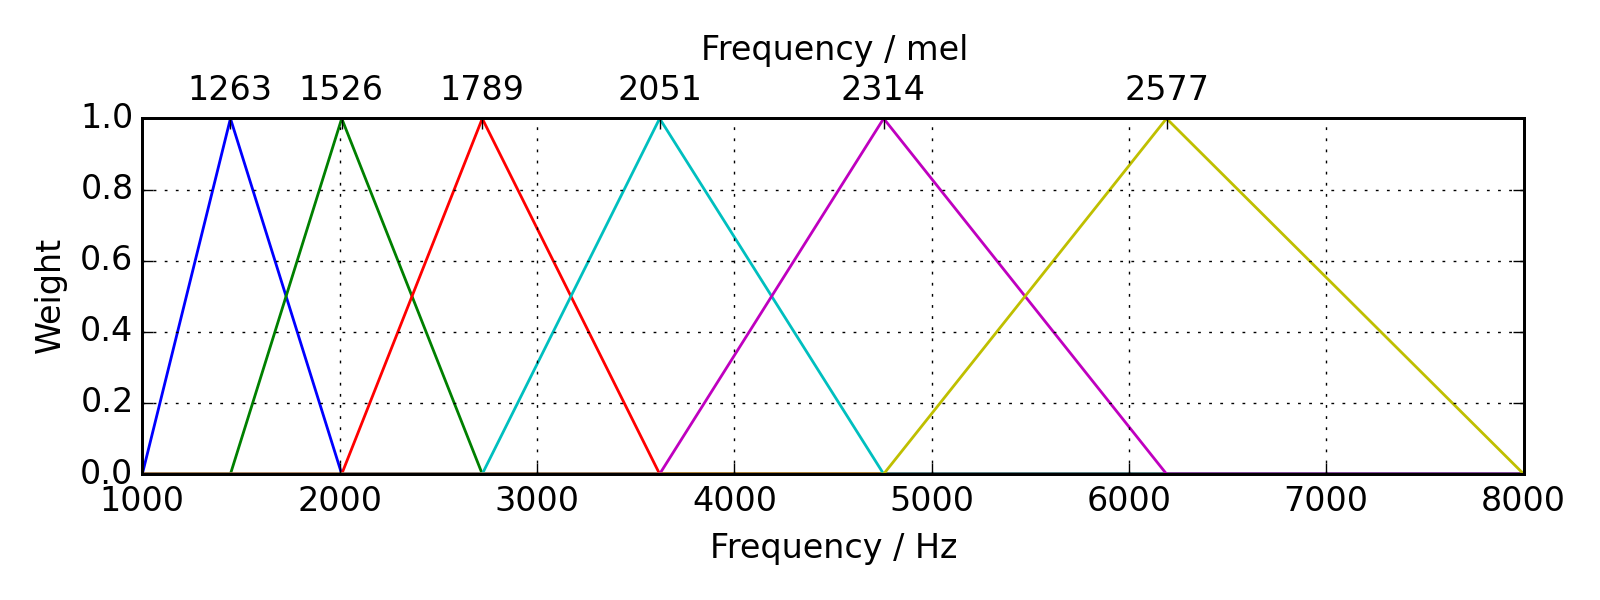
\includegraphics[width=0.8\paperwidth]{mel_filterbank}%
        \caption{Мел скала за $16kHz$ и 6 критични области}
        \label{fig:char:3}
    \end{figure}

    Следващата стъпка е теорията за MFCC коефициенти, която представихме в предния раздел, да влезе в сила . За тази цел, разглеждаме новополучените 23 числа като сигнал.  Правим Фурие трансформация, като запазваме информация само за реалната част (тоест косинуса), тъй като имагинерната част носи ненужната информация за фазата, до получаването на кепстър. Фундаменталната честота на глотиса и хармоничните ѝ ще образуват сигнал, чиято периодичност е засилена от логаритъма. Този ,,сигнал'' е с голяма честота в сравнение със ,,сигнала'', идващ от коефициентите, съответстващи на конфигурацията на вокалния тракт. Затова MFCC коефициентите, отговарящи за него, ще са в по-високите ,,честоти'' на кепстъра.
    Това означава, че не са ни нужни всички MFCC коефициенти, а само тези пред ниските ,,честоти'' на кепстъра. В имплементацията са взети първите 13 MFCC коефициента.

    Изменението на MFCC коефициентите във времето може да донесе допълнителна информация за вокалния тракт и подлежащата емоция. Затова в допълнение на 13-те коефициента, се добавят и първите и вторите им производни по времето.
    Крайният ефект е, че от входния сигнал получаваме за всеки фрейм 39 коефициента, които ще целим да класифицираме.
\end{document}
